\chapter{Synthetic geophysical experiments}

This chapter will outline a series of experiments which will test the main postulate of this thesis, that ABC can offer some improvement over traditional likelihood based Bayesian inference for geophysics. There are many potential avenues to pursue 'improvement'. For example, ABC opens parameter inference to models which were previously closed. This can be used to compare the solution of parameter inference for a stochastic forward where the data and modelization uncertainty do not conform to a Gaussian, to the solution obtained with the simplifying assumption that the uncertainty is Gaussian. This may constitute an improvement in accuracy if it is shown that the ABC solution is significantly different from the analytical Gaussian solution. Instead of pursuing this angle, here I focus explicitly on improving the speed of optimization relative to a general form MCMC sampler. Probabilistic methods which rely on Monte Carlo and MCMC are computationally expensive due to the need to compute the forward at every iteration of the algorithm. As a result the scale of the problems which are computationally tractable is limited. If our limits of understanding about the Earth are to be pushed then it is necessary to develop methods which can tackle large scale problems which are fundamentally defined by solution spaces with uncertainty due to trade-offs between parameters, uncertainty in the experimental data and uncertainty in the modelization process. In this context there is great need for methods which can efficiently find, and then define regions of high probability in very sparse parameter spaces. \par

Here I seek to use the information available by 'opening' the likelihood within each forward simulation to drive improved optimization with ABC, a method which can take into account the full scope of uncertainty in the resulting solution. In this way I abandon the mathematical generality of the applied sampling algorithm in pursuit of one purpose built for the information available within the problem. \par

As with the previous chapter, the code to produce all figures in this section can be found at \url{https://github.com/tomconnell/approximate-bayesian-tomography}.\par


\section{Crustal density inversion}

As a first experiment, I consider an inversion for crustal density ($\rho$) with a vertical gravity anomaly dataset ($\Delta$ g) for a 2D discretized subsurface \citep[p.184-195,378]{blakely1996}. The dimensionality of the parameter space is kept modest, a 8x4 grid, with an observed data point above each column. The grid is defined over a 160 $km$ by 40 $km$ area. The parameter space is bounded between 2-3.5 $g/cm^3$, the limits for which \citet{Brocher2005} define an empirical relationship between density and compressional-wave velocity ($V_p$). This relationship will be used in the next section for a joint inversion. The 'true model', which will be the target of our inversion scheme, is kept smooth to allow a prior term, $p(\bm{\theta})$, to be set for smoothness which will limit the inversion to a unique solution. The definition for smoothness is:
\begin{equation}
-\text{log}\big(p(\bm{\theta})\big) = \sum_{i = 1}^{N} \Big(\sum_{j} (\rho_i - \rho_j)^2\Big)
\label{smoothness}
\end{equation}
where $j$ is a describes all blocks in immediate contact with the given block, $i$. The edge effect for the 2D subsurface grid is compensated by adding the vertical gravity anomaly which will result from extending the grid by a width of one on both sides, tripling the total domain width, with a density which is the average of the parameter space, 2.75 $g/cm^3$. The model is assumed to contain no modelization uncertainty and the data is known to be contaminated with noise defined by $\sigma^{\mathcal{D}} = \mathcal{N}(0,\sqrt{2})$.
\begin{figure}[H]
	\centering
	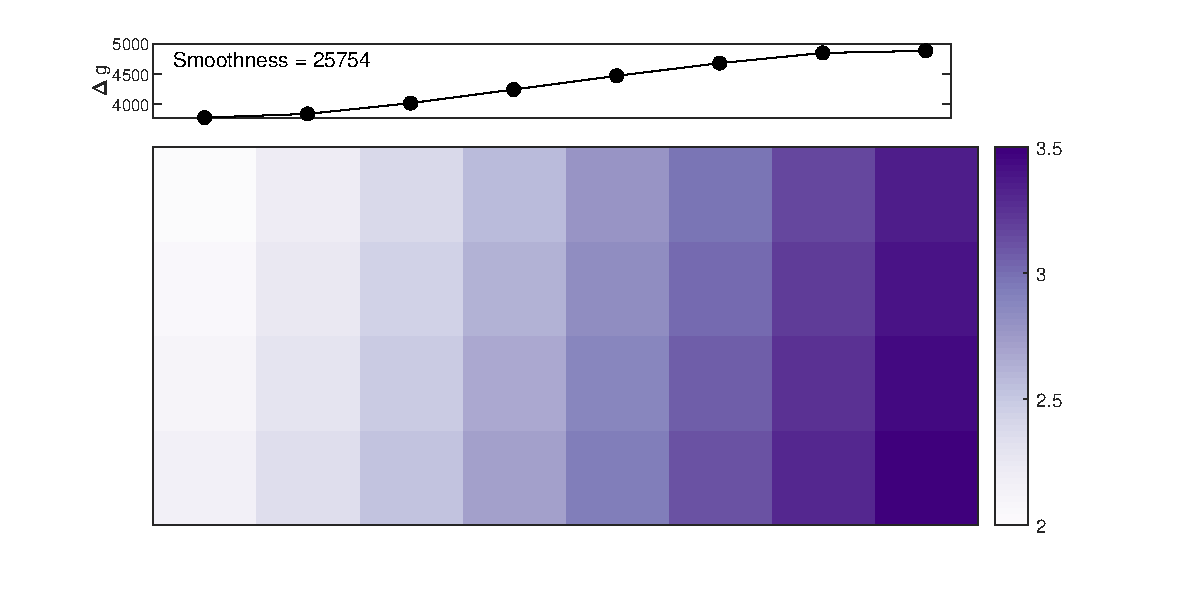
\includegraphics[scale=0.8]{true_model.pdf}
	\caption{The 'observed data', vertical component of gravity ($\Delta g$), and 'true model', a 2D density ($g/cm^3$) slice, which will be the target of our synthetic geophysical experiments to compare ABC to likelihood based Bayesian inference. A smoothness value, log($p(\bm{\theta})$), equation \ref{smoothness}, for the true model is plotted for reference to later solutions.}
	\label{true_model}
\end{figure}
The benchmark for ABC-tomography to meet will be MCMC sampling of an analytically defined posterior. Given there is no modelization uncertainty and $\sigma^{\mathcal{D}}$ is known, the negative log-likelihood can be defined by, equation \ref{likelihood-1}:
\begin{equation}
	-l(\bm{\theta^*}|\bm{y}) = \frac{(\bm{y}-\bm{y^*})^2}{(\sigma^{\mathcal{D}})^2}
	\label{analytical-applied-likelihood}
\end{equation}
For this section only MCMC is considered, no AM, DR or DRAM. This maintains a consistent sampling benchmark for comparison to the ABC scheme. The proposal distribution for both MCMC sampling of the analytical distribution and ABC-tomography is held constant for all runs as $q(\cdot,\cdot) = \mathcal{N}(0,I\cdot250)$. The parameter space is subdivided into eight 2x2 blocks. At each time step a random block is selected in the subsurface and updated via $q(\cdot,\cdot)$. As demonstrated in table \ref{sampling-method-comparison}, the number of parameters updated at each time step impacts the acceptance rate and the rate of space exploration of the chain. To keep inference comparable both the analytical scheme and ABC scheme will update 4 parameters per time step via the proposal distribution. Likewise, for each experiment considered in this section the Markov chain starting position is the same for both the analytical and ABC-tomography. The starting position for both is set by sampling a uniform distribution, $\mathcal{U}(2,3.5)$, to define each unknown parameter. \par
A set of summary statistics to describe the data in Figure \ref{true_model} is needed to proceed with ABC-tomography. Here I seek safety in a comprehensive description of the data by the co-efficients to a linear model, $m$ and $b$, the sample mean, $\bar{\mu_{\Delta g}}$, sample standard deviation, $\bar{\sigma_{\Delta g}}$, and a failsafe residual term, $\sum R$, for the difference between a simulation and the observed data for a given $\bm{\theta^*}$, $R = |\bm{y}-\bm{y^*}|$. Initial testing showed the set of statistics $\begin{bmatrix}
\bar{\mu_{\Delta g}}\ \bar{\sigma_{\Delta g}}\ m\ b\ \sum R
\end{bmatrix}^T$ comprehensively describes $\bm{y}$. As with section \ref{banana-section}, it is necessary to normalize the spread of each marginal distance term, $\text{d}_i(S_i(\bm{y}),S_i(\bm{y^*}))$, equation \ref{marginal_distance}, to one. This accounts for the different scales and sensitivities of the summary statistics to the unknown parameters. The normalization term $\bm{\sigma_S}$ is approximated from >10,000 Monte Carlo simulations over parameter range 2-3.5 $g/cm^3$. The tolerance is closely related to the acceptance rate of the algorithm. Given the tolerance is tightly tied to the acceptance rate, the tolerance is tuned to give a reasonable acceptance rate (approx. 20\%).\par
For the ABC-tomography scheme I am free to open the likelihood, consider the information available, and use that to drive the next step in the Markov chain. As a first adjustment I localize the updates to directly below a data point, and choose which column of parameters to transition based on a probability distribution proportional to the misfit between the observed data $\bm{y}$, and the simulated data set $\bm{y^*}$. Here and throughout misfit is defined by the l2-norm:
\begin{equation}
	\text{misfit} = (\bm{y}-\bm{y^*})^2
	\label{misfit}
\end{equation}
The effectiveness of dynamically selecting and localizing the updates relies on our physical intuition about the relationship between the unknown model parameters and the resulting data. In this case, the each simulated data point is most sensitive to the parameters which are directly below it, and by focusing model updates on regions which are poorly fitting, the most is made from each move during the initial optimization phase in finding areas of high posterior probability density. This change has ideas similar to the way gradient-based linear optimization methods work, however, here I simply rely on physical intuition within a Bayesian fully probabilistic framework. \par
Figure \ref{comparison-1} plots a comparison between the misfit, equation \ref{misfit}, for the analytical scheme described above and ABC-tomography during the optimization phase of the respective Markov chains (first 10,000 time steps). The localization of parameter updates to areas where the current model is a poor fit increases the speed of optimization. Figure \ref{ana-im-1} and \ref{abc-im-1} plot the solution obtained, mean marginal model, for the full chain (100,000 time steps).\par

\begin{figure}[H]
	\centering
	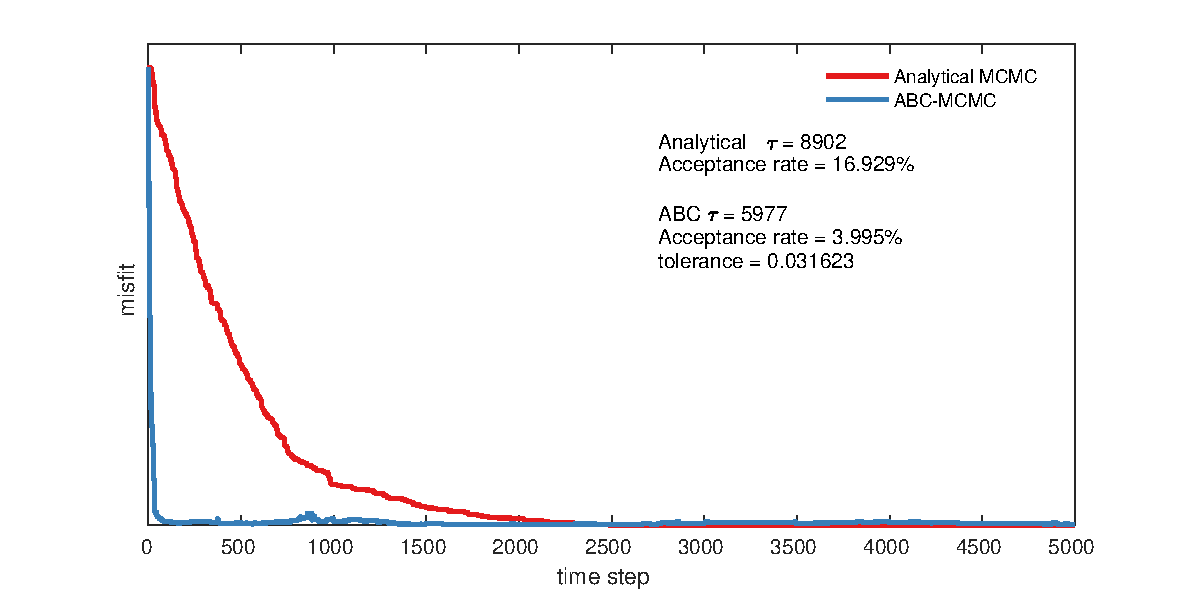
\includegraphics[scale=0.8]{comparison.pdf}
	\caption{The misfit, l2-norm, equation \ref{misfit}, for the chain state during the optimization phase (first 10,000 time steps) for an analytically defined posterior compared to ABC-tomography. The 'true model' and observed data is plotted in figure \ref{true_model}. Both posteriors, analytical and ABC-tomography, use a parameter space bound between 2-3 $g/cm^3$ and a prior 'smoothness' defined by equation \ref{smoothness}. The speed increase in optimization is a result of opening the likelihood and using the information contained in each iteration to localize the next update to an area where the current data fit is poor. The details of the full chain run, 100,000 time steps, are also displayed on the figure. $\tau$ is the integrated auto-correlation time.}
	\label{comparison-1}
\end{figure}

\begin{figure}[H]
	\centering
	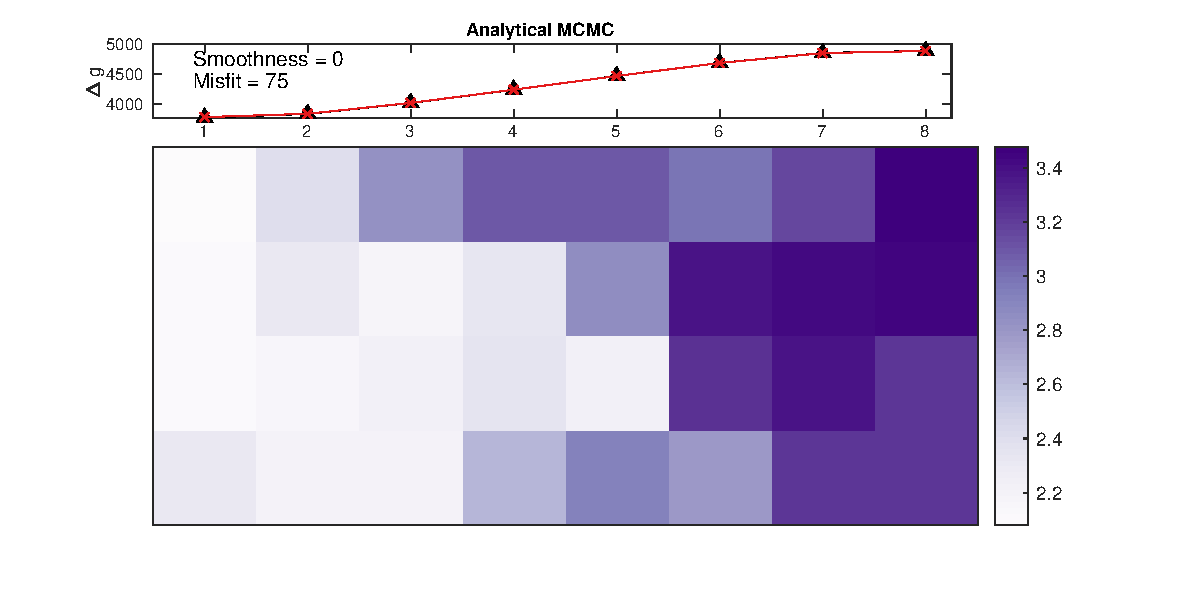
\includegraphics[scale=0.8]{ana_im.pdf}
	\caption{The mean of the marginal posterior, $p(\bm{\theta}|\bm{y})$, defined by the prior equation \ref{smoothness} and likelihood \ref{analytical-applied-likelihood} targeting the 'true model' and observed data of figure \ref{true_model}. The simulated data generated by this 'solution' is plotted, red, compared to the observed data, black. The smoothness, equation \ref{smoothness}, and misfit, equation \ref{misfit}, for this model are displayed alongside the data. The misfit during the optimization phase for this chain is plotted in figure \ref{comparison-1}. This model can be compared to the equivalent for the ABC-tomography chain.}
	\label{ana-im-1}
\end{figure}

\begin{figure}[H]
	\centering
	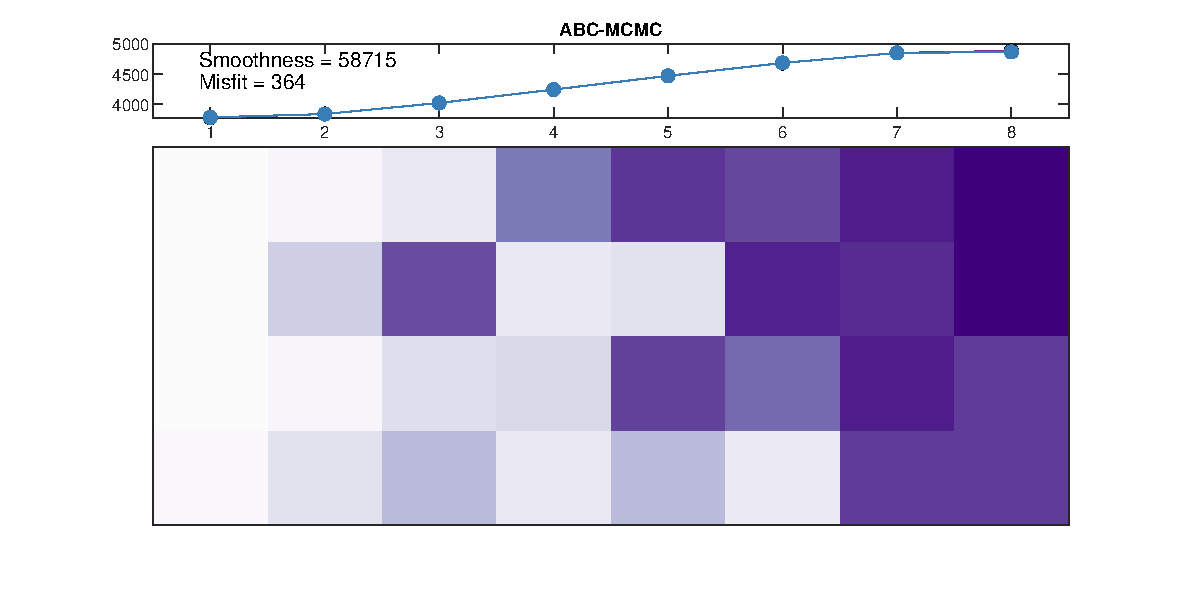
\includegraphics[scale=0.8]{abc_im.pdf}
	\caption{The mean of the marginal ABC posterior, $p_{ABC}(\bm{\theta}|\bm{S}(\bm{y}))$, targeting the 'true model' and observed data of figure \ref{true_model}. The simulated data generated by this 'solution' is plotted, blue, compared to the observed data, black. The smoothness, equation \ref{smoothness}, and misfit, equation \ref{misfit}, for this model are displayed alongside the data. The misfit during the optimization phase for this chain is plotted in figure \ref{comparison-1}. This model can be compared to the equivalent for the analytically defined posterior.}
	\label{abc-im-1}
\end{figure}

\citet{Sisson2010a} highlight that sampler acceptance rate and mixing can be improved by increasing the number of simulated datasets, $\bm{y^*}$, for each set of model parameters, $\bm{\theta^*}$. This is a technique also adopted in applications with large uncertainty in $\bm{g_s}$ \citep{Ratmann2009,Wood2010}. This has a large stabilizing impact when the uncertainty in each simulation is large. Here I adopt this technique for $k = 100$ simulations from $\bm{g_s}$. Since the bulk of the computational overhead is in solving the deterministic physical model and the data uncertainty is additive and fast to simulate, there is little computational cost in increasing  the number of simulated datasets. The distance is then computed based the sample mean of $\bm{y^*_{1:k}}$, $\bm{d} = |\bm{S}(\bm{y})-\bm{S}(\bm{\bar{\mu_{y^*}}})|$.


\section{Crustal density joint inversion}

As a second experiment I extend the inversion for crustal density ($\rho$) for a 2D discretized subsurface to a joint inversion with vertical gravity anomaly ($\Delta$ g) and travel times for compressional-waves $V_p$. Both datasets share the same underlying parameter space in $\rho$. The calculation for $V_p$ is made through the empirical relationship for $V_p$ as a function of $\rho$ defined by \citet{Brocher2005}:
\begin{equation}
	V_p\ (km/sec) = 0.8228\rho^5 - 9.1819\rho^4 + 37.0.83\rho^3 - 63.064\rho^2 + 39.128\rho
	\label{rhotovp}
\end{equation}
This relationship is valid for crustal rocks with $\rho$ in the range of 2-3.5 $g/cm^3$. As with the first example the 'true model' is kept smooth and the prior \ref{smoothness} is used. The parameter space is expanded to a 20x6 grid over the same 160 $km$ by 40 $km$ area. There is a $\Delta$ g measurement made above each fo the 20 columns. Both the $\Delta$ g and $V_p$ dataset are contaminated with measurement uncertainty defined by $\sigma^{\mathcal{D}} = \mathcal{N}(0,\sqrt{2})$. As before, the benchmark for ABC-tomography will be MCMC sampling of an analytically defined posterior. The likelihood for this problem is based on \ref{joint-likelihood}, with a negative log-likelihood defined as:
\begin{equation}
	-l(\bm{\theta}|\bm{y}) = \frac{c(\bm{y_{\Delta g}}-\bm{y^*_{\Delta g}})^2}{(\sigma^{\mathcal{D}})^2} + \frac{(\bm{y_{V_p}}-\bm{y^*_{V_p}})^2}{(\sigma^{\mathcal{D}})^2}
\end{equation}
where $c$ is a constant defined so as the contribution to the negative log-likelihood of both datasets is of the same order of magnitude. The proposal distribution is held as $q(\cdot,\cdot) = N(0,I\cdot250)$ however, given the increased parameter space the subsurface is divided into 20 2x3 blocks. A random block is selected for update at each time step in the analytical scheme. The starting position is initialized from $\mathcal{U}(2,3.5)$  and once again held constant between both the analytical Markov chain and ABC-tomography. \par

I once again seek a comprehensive set of summary statistics to describe $\bm{y_{\Delta g}}$ and $\bm{y_{V_p}}$. The set $\begin{bmatrix}
\bar{\mu_{\Delta g}}\ \bar{\sigma_{\Delta g}}\ m\ b\ \sum R
\end{bmatrix}^T$ is used for $\bm{y_{\Delta g}}$. Given $\bm{y_{V_p}}$ is the vector for arrival times for each source. Instead of fitting statistics to the larger $\bm{y_{V_p}}$, $\bm{y_{V_p}}$ is decomposed to the set of data for each source, 1 to $l$, where $l$ is the number of sources. The arrivals from each individual source are then described by $\begin{bmatrix}
m\ b\ \sum R
\end{bmatrix}^T$. The weighting kernel for $\bm{y_{V_p}}$ then becomes:
\begin{equation}
	p(\bm{y_{V_p}}|\bm{y^*_{V_p}},\bm{\theta^*}) = \prod_{i = 1}^{l} p(\bm{y_i}|\bm{y^*_i},\bm{\theta^*})
\end{equation}
A normalization term $\bm{\sigma_S}$ is approximated for both datasets from >10,000 Monte Carlo simulations over parameter range 2-3.5 $g/cm^3$. \par

For ABC-tomography I again open the likelihood at each time step and consider the information available to localize the parameter updates. The 6 parameters below a given data point are updated based on Monte Carlo sampling of a probability distribution proportional to the misfit of the $\bm{y_{\Delta g}}$ data set. For this joint inversion I extend the ABC-tomography scheme based on physical intuition by both dynamically selecting and localizing the update, and directing proposal to bias the update in the direction which the data needs to go. This is done through the use of a skew normal distribution or alternatively a truncated Gaussian distribution. These distributions are then adjusted to bias the update in either a positive or negative direction. If, for example, a gravity anomaly is selected by sampling the misfit distribution and it is found to be too large, i.e the value $y^*_{\Delta g} - y_{\Delta g}$ is positive, then the proposal for the column of parameters at this update step can be either sampled from: a negatively skewed normal distribution centered on the current chain position; or a truncated normal distribution, which is truncated at some position greater than the current chain position. An example of the proposals used in this example to negatively or positively bias the proposal distribution is plotted in Figure \ref{updates}. \par
It should be noted that when using the skew normal distribution, as it is not a symmetric distribution, the ratio $\frac{q(\bm{\theta^*},\bm{\theta_{t-1}})}{q(\bm{\theta_{t-1}},\bm{\theta^*})}$ must be computed at each time step. \par

\begin{figure}[H]
	\centering
	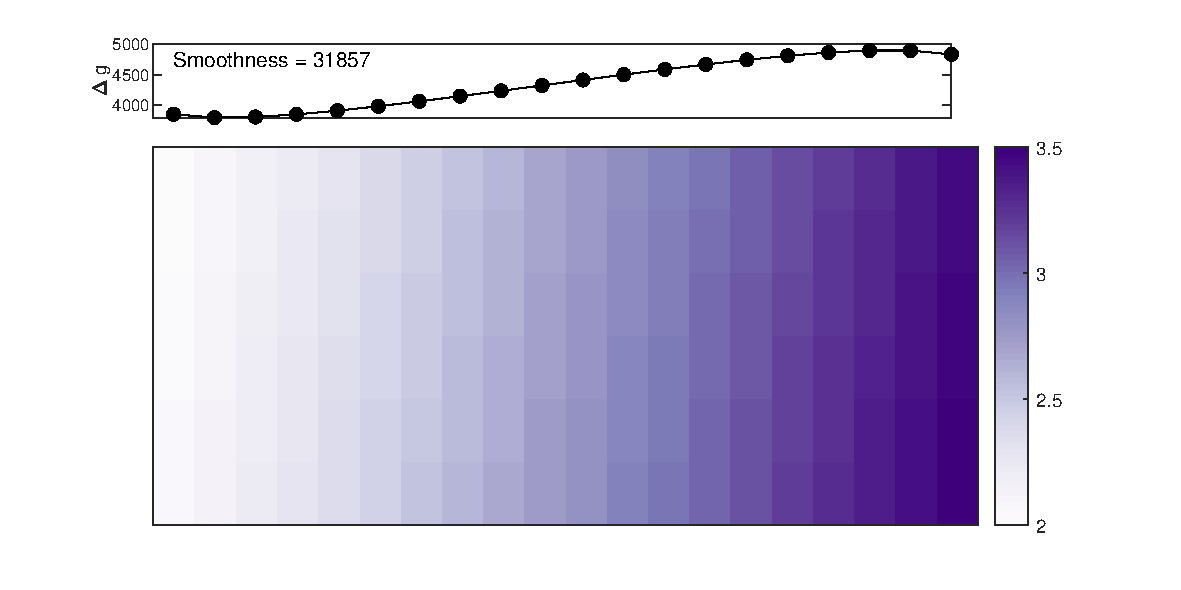
\includegraphics[scale=0.75]{true_model_gravity.pdf}
	\caption{The 'observed data', vertical component of gravity ($\Delta g$), and 'true model', a 2D density ($g/cm^3$) slice, which will be the target of our synthetic geophysical experiments to compare ABC to likelihood based Bayesian inference. A smoothness value, log($p(\bm{\theta})$), equation \ref{smoothness}, for the true model is plotted for reference to later solutions.}
	\label{true-model-large-grav}
\end{figure}

\begin{figure}[H]
	\centering
	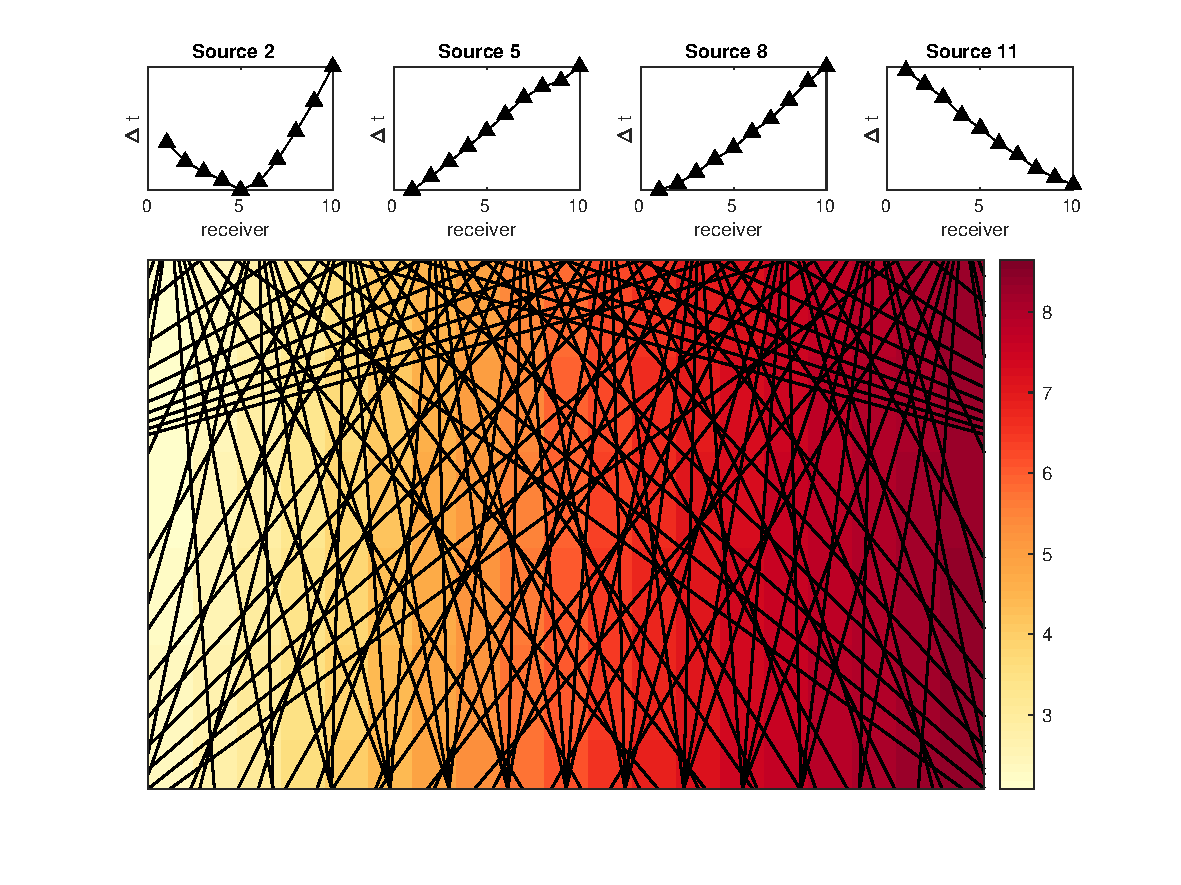
\includegraphics[scale=0.75]{observed_tomography.pdf}
	\caption{The 'true model', a 2D $Vp$ ($km/s$) slice, converted from $\rho$ by the empirical relationship defined by equation \ref{rhotovp}. The black lines across the model define the rays from 12 sources on their path to 10 receivers. The arrival time $\Delta t$ of these rays at the receivers defines the 'observed data'. A sample of observed data is plotted for 4 sources. The sources are numbered 1-12 starting from the top left and going to the top right, with 4 sources per side.}
	\label{true-model-tom}
\end{figure}


The analytical definition for the skew normal distribution, $f(x)$, used to direct the parameter updates is:
\begin{equation}
\begin{split}
\phi(x) = \frac{1}{\sqrt{2\pi}}\text{exp}\Big(-\frac{x^2}{2}\Big) \\
\Phi(x) = \frac{1}{2}\bigg(1 + \text{erf}\Big(\frac{x}{\sqrt{2}}\Big)\bigg)\\
f(x) = \frac{2}{\omega} \phi\bigg(\frac{x-\xi}{\omega}\bigg)\Phi\bigg(\alpha \Big(\frac{x-\xi}{\omega}\Big)\bigg)
\end{split}
\label{skew-normal-dist}
\end{equation}
here erf is the error function, $\xi$ is the location, $\omega$ is the scale and $\alpha$ is a shape parameter. In this application  $\xi$ is the current chain location, $\omega$ is held at 250, and $\alpha$ is either 1, for a positively skewed distribution, or -1, for a negatively skewed distribution. \par
The analytical definition for the truncated normal distribution, $f(x)$, used to direct the parameter updates is:
\begin{equation}
	f(x) = \begin{cases} 
	0 & x < a \\
	\frac{1}{\sqrt{2\pi\sigma^2}}\text{exp}\Big(-\frac{(x-\mu)^2}{2\sigma^2}\Big) & a\leq x\leq b \\
	0 & x > b 
	\end{cases}
	\label{trunc-eq}
\end{equation}
Here $a$ is the lower cut-off and $b$ is the upper cut-off. In this application the negatively truncated distribution has $a = -\frac{1}{2}\sigma$ and $b = \infty$. While the positively truncated distribution has $a = -\infty$ and $b = \frac{1}{2}\sigma$. For our application $\mu$ is the current chain location and $\sigma$ = 250. \par
Figure \ref{updates} plots the directed proposal distributions described above and applied in ABC-tomography. Figure \ref{updates}(a)(b) are used when the parameter values need to be lowered, and figure \ref{updates}(c)(d) are used when the parameter values need to be increased. 

\begin{figure}[H]
	\centering
	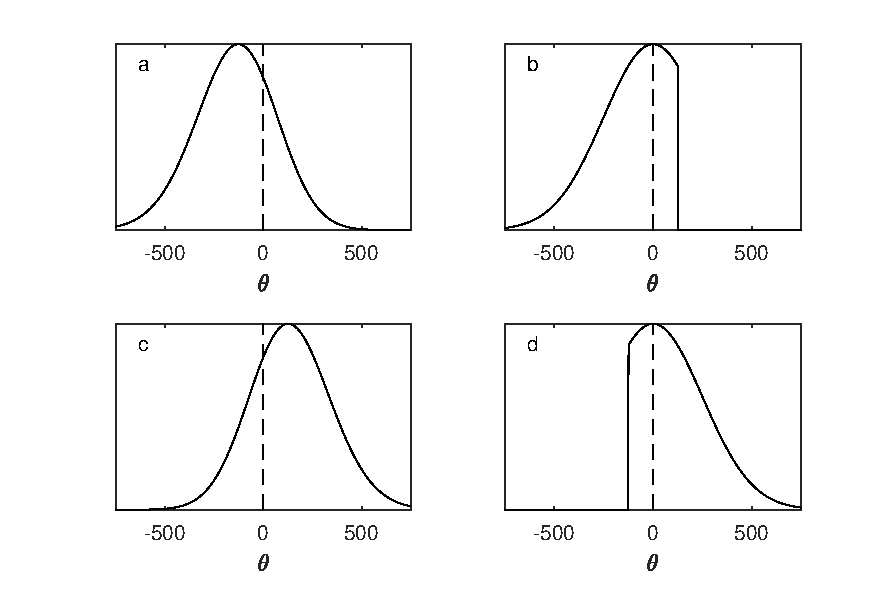
\includegraphics[scale=1]{updates.pdf}
	\caption{The proposal distributions which are used to either positively or negatively bias the parameter update. The negatively skewed Gaussian distribution in (a) and the positively truncated Gaussian distribution in (b) are used to bias the proposal when the parameter values are deemed too high. The positively skewed Gaussian distribution (c) and the negatively truncated Gaussian distribution when the parameter values are deemed too low. Equation \ref{skew-normal-dist} defines the skew Gaussian distribution while equation \ref{trunc-eq} defines the truncated Gaussian distribution. During application the distributions are centered on the current chain position, and $\sigma = \omega = 250.$. The shape parameter, $\alpha$, and cut-off, $a$ and $b$ are selected to set the bias at approximately 70\% to 30\%.}
	\label{updates}
\end{figure}

Figure YY and ZZ plots a comparison between the normalized misfit for the analytical scheme and ABC-tomography during the optimization phase of their respective Markov chains for both skew normal and truncated normal updates. This shows how the speed of optimization can be improved through opening the likelihood and allowing the simulated data to select, localize and direct the parameter updates. While it should be noted that the acceptance rate collapses when compared to undirected ABC-tomography, each move is more informed and the quality of next move in the chain is higher (i.e the misfit is lower). Figure AA, BB, CC, and DD plot the mean marginal model for the full chain lengths. This demonstrates the accuracy of the recovered solutions. \par



